%%%%%%%%%%%%%%%%%%%%%%%%%%%%%%%%%%%%%%%%%%%%%%%%%%%%%%%%%%%%%%%
%%%  SFC = superfluidity and chaos
%%%%%%%%%%%%%%%%%%%%%%%%%%%%%%%%%%%%%%%%%%%%%%%%%%%%%%%%%%%%%%%

% For submission redefine \rmrk \hrefl \hidea

\documentclass[aps,pre,floats,floatfix,twocolumn]{revtex4-1}
%\documentclass[fleqn,10pt]{wlscirep}

% special 
\usepackage{ifthen}
\usepackage{ifpdf}
\usepackage{color}

\ifpdf
\usepackage{graphicx}
\usepackage{epstopdf}
\else
\usepackage{graphicx}
\usepackage{epsfig}
\fi
\graphicspath{{./Figs_SBM_jpg/}{./}}

% fonts
\usepackage{latexsym}
\usepackage{amsmath}
\usepackage{amssymb}
\usepackage{bm}
\usepackage{wasysym}

\usepackage{mathptmx}
\DeclareSymbolFont{epsilon}{OML}{ntxmi}{m}{it}
\DeclareMathSymbol{\epsilon}{\mathord}{epsilon}{"0F}

\usepackage{hyperref}

% Standard symbols 
\newcommand{\sinc}{\mbox{sinc}}
\newcommand{\const}{\mbox{const}}
\newcommand{\trc}{\mbox{trace}}
\newcommand{\intt}{\int\!\!\!\!\int }
\newcommand{\ointt}{\int\!\!\!\!\int\!\!\!\!\!\circ\ }
\newcommand{\ar}{\mathsf r}
\newcommand{\im}{\mbox{Im}}
\newcommand{\re}{\mbox{Re}}

% Special symbols
\newcommand{\mass}{\mathsf{m}} 
\newcommand{\Mass}{\mathsf{M}} 

% Math constractions
\newcommand{\tbox}[1]{\mbox{\tiny #1}}
\newcommand{\bmsf}[1]{\bm{\mathsf{#1}}} 
\newcommand{\amatrix}[1]{\begin{matrix} #1 \end{matrix}} 
\newcommand{\eexp}[1]{\mathrm{e}^{#1}}
\newcommand{\pd}[2]{\frac{\partial #1}{\partial #2}}
\newcommand{\bra}[1]{\left\langle #1 \right|}
\newcommand{\ket}[1]{\left| #1 \right\rangle}
\newcommand{\braket}[1]{ \left\langle #1 \right\rangle}
\newcommand{\Braket}[2]{ \left\langle #1 \middle| #2 \right\rangle}
\newcommand{\BraKet}[3]{ \left\langle #1 \middle| #2 \middle| #3 \right\rangle}
\newcommand{\avg}[1]{\left\langle #1 \right\rangle}
\newcommand{\ola}{\protect\overleftarrow}
\newcommand{\ora}{\protect\overrightarrow}

% Equations
\newcommand{\be}[1]{\begin{eqnarray}\ifthenelse{#1=-1}{\nonumber}{\ifthenelse{#1=0}{}{\label{e#1}}}}
\newcommand{\beq}{\begin{eqnarray}}
\newcommand{\eeq}{\end{eqnarray}} 

% Text arrangement
\newcommand{\hide}[1]{}

\newcommand{\Eq}[1]{\textcolor{blue}{{equation}\!~(\ref{#1})}} 
\newcommand{\Fig}[1]{\textcolor{blue}{Fig.}\!\!~\ref{#1}}
\newcommand{\sect}[1]{{\bf #1.-- }}
\newcommand{\drawline}{\begin{picture}(500,1)\line(1,0){500}\end{picture}}
\newcommand{\bitem}{$\bullet$ \ \ \ }
\newcommand{\Cn}[1]{\begin{center} #1 \end{center}}
%\renewcommand{\cite}[1]{\textcolor{blue}{[\onlinecite{#1}}]} %{[\onlinecite{#1}]} 



% temporary turn off figures
%\renewcommand{\includegraphics}[2][]{{\color{blue} \hspace{1cm} --FIGURE-- \hspace{1cm} }}

\newcommand{\rmrk}[1]{{#1}}     %{\textcolor[rgb]{0.6,0,0.1}{#1}}
\newcommand{\hrefl}[1]    {\href{#1}{[link]}}
\newcommand{\hidea}[1]{}    %{{#1}}


%%%%%%%%%%%%%%%%%%%%%%%%%%%%%%%%%%%%%%%%%%%%%%%%%%%%%%%%%%%%%%%%%%%%%%%%%%%%%%%%%%%%%%%%%%
%%%%%%%%%%%%%%%%%%%%%%%%%%%%%%%%%%%%%%%%%%%%%%%%%%%%%%%%%%%%%%%%%%%%%%%%%%%%%%%%%%%%%%%%%%
\begin{document}
 
\title{Percolation, sliding, localization and relaxation in glassy circuits}

\author{DH and DC}

\affiliation{Department of Physics, Ben-Gurion University of the Negev, Beer-Sheva, Israel}

%%%%%%%%%%%%%%%%%%%%%%%%%%%%%%%%%%%%%%%%%%%%%%%%%%%%%%%%%%%%%%%%%%%%%%%%%%%%%%%%%%%%%%%%%%
%%%%%%%%%%%%%%%%%%%%%%%%%%%%%%%%%%%%%%%%%%%%%%%%%%%%%%%%%%%%%%%%%%%%%%%%%%%%%%%%%%%%%%%%%%

%\begin{abstract}
%\end{abstract}

\maketitle
%
%
%There is a recent interest in ``glassy" systems that have log-wide distribution of 
%relaxation rates. For example we note recent works regarding electron dynamics where 
%the effective model is essentially the same as {\em random walk in disordered lattice}. 
%In such type of model there is a percolation-related crossover to sub-diffusion (in one dimension), 
%or to variable-range-hopping type diffusion (in general). 
%This crossover is reflected in the spectral properties of the system.
%%
%The more general problem of {\em random walk in random environment}, 
%where transitions between sites are allowed to be asymmetric, 
%has been explored by Sinai, Derrida, and followers. 
%Focusing on one-dimensional systems, it turns out that 
%for any small amount of disorder an unbiased spreading 
%becomes sub-diffusive. For bias that exceeds a non-zero threshold there 
%is a {\em sliding transition}, and the drift velocity becomes non-zero.
%%
%Considering an $N$-site ring geometry, we ask what are the implications 
%of the percolation and of the sliding transitions on the relaxation modes 
%of such topologically closed system. A complementary question regarding  
%the ``delocalization" of eigenstates of non-Hermitian quantum Hamiltonians
%has been addressed by Hatano, Nelson, and followers. 
%We show below that for a conservative "random walk" dynamics 
%the implied spectral properties are dramatically different.
%  
  
  

There is recent interest in ``glassy" systems that have log-wide distribution of 
relaxation rates \cite{glass1}. For example we note recent works regarding electron dynamics where 
the effective model is essentially the same as a {\em random walk on a disordered lattice} \cite{ege,egt}. 
In such type of model there is a percolation-related crossover to sub-diffusion (in one dimension), 
or to variable-range-hopping type diffusion (in general) \cite{pts,}. 
This crossover is reflected in the spectral properties of the system.
An equivalent point of view regarding percolation is the continuous time random walk (CTRW) with
a broad distribution of waiting times \cite{BouchaudReview}.
%
The more general problem of {\em random walk in random environment}, 
where transitions between sites are allowed to be asymmetric, 
has been explored by Sinai \cite{Sinai}, Derrida \cite{odh1}, and followers \cite{odh3,BouchaudReview}. 
Focusing on one-dimensional systems, it turns out that 
for any small amount of disorder an unbiased spreading 
becomes sub-diffusive. For bias that exceeds a non-zero threshold there 
is a {\em sliding transition}, and the drift velocity becomes non-zero.
%
Considering an $N$-site ring geometry, we ask what are the implications 
of the percolation and of the sliding transitions on the relaxation modes 
of such topologically closed system. A complementary question regarding  
the ``delocalization" of eigenstates of non-Hermitian quantum Hamiltonians
has been addressed by Hatano, Nelson, and followers \cite{Hatano1,Hatano2, Shnerb1}. 
Their main achievement is the realization that the complex spectrum of the non-Hermitian hamiltonian 
can be deduced from the real spectrum of an associated Hermitian hamiltonian. 
Various improvements on the method and ensuing analytical results were obtained.
For example, the complex spectrum in the thermodynamic limit was found in \cite{Brouwer}.
An equation for the curve in the complex plane on which the eigenvalues are located and the density of states was found in \cite{Goldsheid}.
Results for special models of one impurity and one way dynamics (maximally asymmetric transition rates) were obtained in \cite{Zee}.
The physical phenomena that inspired this line of work is vortex depinning in type II superconductors \cite{Hatano1,Hatano2}, yet parallels to non quantum systems were drawn. Such systems include pulling pinned polymers, DNA denaturation \cite{DNA1,DNA2} and non conservative population biology \cite{popbio}.
%
We show below that for a conservative "random walk" dynamics 
the implied spectral properties are dramatically different.
%  
Notable "conservative random walkers" are Brownian motors. For example, molecular motors on heterogeneous tracks, such as DNA or RNA \cite{brm1,brm2}. It was found that under an external force and strong disorder, the motor will become localized at preferred positions yet near the stall force, localization occurs for any amount of disorder. These results were obtained by observing the numerically obtained spectrum. 

To summarize \cite{brm2}, they use a different method, bypassing the hermitization procedure.
The long time behavior of $v$ and $D$ is deduced by numerical observations of the lower edge of the spectrum (small $|\lambda|$).
In fact the hermitization procedure is claimed to obscure the complexity (we found it!).
Somehow they do not bridge between complexity of the spectrum and the sliding transition in a purely conservative model. 
They make some comments regarding complexity and sliding in the following respect.
They consider a model where there are two types of unit cells. Each unit cell is made of two bonds.
The chain is composed of unit cells drawn from a bimodal distribution. 
Real eigenvalues only appear due to non conservative diagonal disorder  (detachment rate).
They do not find an explicit crossover to complexity and do not handle the purely conservative case.
% In which case, they do make a connection with Derrida. They study the complexity vs. disorder in the detachment rate. 
%For $\mu>1 $, for weak disorder the spectrum is complex, for strong disorder there are real eigenvalues. 
%Form $\mu<1$, there are real eigenvalues even for very small disorder.

%%%%%%%%%%%%%%%%%%%%%%%%%%%%%%%%%%%%%%%%%%%%%%%%%%%%%%%%%%%%%%%%%%%%%%%%%%%%%%%%%%%%%%%%%%%%%%%%%%%%%%%%%%%%%%%%%%%%
\section{Stochastic spreading}

%%%%%%%%%%%%%%%%%%%%%%%%%%%%%
\sect{Diffusive spreading}
%
Einstein has considered in his thesis the problem of Brownian motion. 
This can be regarded as a stochastic process in which a particle hops from site to site with some hopping rate~${w}$. The rate equation can be written in matrix notation as 
%
\be{1}
\frac{d\bm{p}}{dt} \ \ = \ \ \bm{W} \bm{p}, 
\eeq
%
involving a matrix ${\bm{W}}$ whose off-diagonal elements are the transitions rates ${w_{nm}}$, 
and with diagonal elements ${-\gamma_n}$ such that each column sums to zero. 
For example, in the case of a one-dimensional lattice with near-neighbor hopping
%
\be{2}
\bm{W} \ \ = \ \ \left[\amatrix{
-\gamma_1   & w_{1,2}   & 0         & ... \\ 
w_{2,1}     & -\gamma_2 & w_{2,3}   & ... \\ 
0           & w_{3,2}   & -\gamma_3 & ... \\
...         & ...       & ...       & ...
}\right]
\eeq 
%
with ${\gamma_n=\sum_{m (\neq n)} w_{mn}}$.
Einstein's theory assumes a symmetric matrix $\bm{W}$.   
The diffusion coefficient is ${D\sim wa^2}$, 
where $w$ is the average hopping rate between neighboring sites, 
and $a$ is the average distance between them.  
The associated negative eigenvalues ${\{-\epsilon_k\}}$ of the matrix $\bm{W}$ 
are characterized by the spectral density 
%
\be{3}
\rho(\epsilon) = \const \ \epsilon^{\mu-1} \ \ \ \ \text{(for small $\epsilon$)}
\eeq
%
where ${\mu=d/2}$, and ${d=1,2,3}$ is the dimensionality. 
It is physically appealing to think of $\bm{W}$ as the 
Hamiltonian matrix of a particle on a lattice, 
and then ${-\epsilon_k}$ are the eigen-energies. 
Optionally the $w_{nm}$ may represent spring-constants, 
and then ${\omega_k=\sqrt{\epsilon_k}}$ are the Debye 
frequencies of the vibrational modes. 


%%%%%%%%%%%%%%%%%%%%%
\sect{Percolation transition}
%
The first question that arises is how is Einstein's result affected if the rates come from some wide distribution. The simplest model assumes randomly distributed sites, and rates that depend exponentially on the distance ${w\propto \exp(-r/\xi)}$. For such a type of model the distribution of the rates is 
%
\beq
P(w) = \const \ w^{\alpha-1} \ \ \ \ \text{(for small $w$)}
\eeq
%
where ${\alpha=\xi/a}$. If the distance between the sites is increased, $\alpha$ decreases. 
As the network becomes ``glassy" (${\alpha<1}$) there is a percolation-related transition 
to very slow diffusion (``variable range hopping"). This holds for any dimension ${d>1}$. 
For one dimension ($d=1$) there is a more dramatic transition to sub-diffusion. 
In the later case the spectral density is no longer ${\mu=d/2=1/2}$, but 
%
\beq
\mu [\text{of symmetric matrix}] \ \ = \frac{\alpha}{1+\alpha} \ \ \leq  \ \ 1/2 
\eeq  


%%%%%%%%%%%%%%%%%%%%%%%
\sect{Sinai spreading}
%
The second question that arises is what happens to Einstein's theory if the transition rates are asymmetric.
This question has been addressed by Sinai, Derrida and followers, 
sometimes called "random walk in random environment". We define the stochastic field as
%
\be{6}
\mathcal{E}_{m \leadsto n} \ \ \equiv \ \ \ln\left(\frac{w_{nm}}{w_{mn}}\right), \ \ \ \ \ \ \  (n \neq m)   
\eeq
%
such that the ratio of "backward" to "forward" transitions equals a Boltzmann factor ${\eexp{-\mathcal{E}}}$. 
For the purpose of presentation we assume that the stochastic field has box distribution within ${[s-\sigma,s+\sigma]}$. 
The average value~$s$, the so called affinity, determines the direction of the drift velocity~$v=v_{\sigma}(s)$. 
It is well known that by a similarity transformation the~$\bm{W}$ of an {\em open} chain becomes a symmetric matrix~$\bm{H}$.     
The associated spectrum ${\{-\epsilon_k\}}$ consist of real negative values, and is characterized by 
a spectral density $\rho(\epsilon)$ that is discussed below.   


%%%%%%%%%%%%%%%%%%%%%%%
\sect{Sliding transition}
%
Consider a sample of $N$ sites. For~${s\ll 1/N}$ the Einstein relation implies that $v/D=s$. 
For larger~$s$ the ratio becomes smaller, and eventually for a very large~$s$ it saturates $v/D\rightarrow 2/a_{\sigma}$.  
The length scale~$a_{\sigma}$ depends on the disorder~$\sigma$, and equals the lattice constant 
in the absence of disorder (${a_0=a}$). 
%
In the limit $N\rightarrow\infty$ it has been established that $v_{\sigma}(s)=0$ 
up to some critical value~${s_1}$. For ${s>s_1}$ the drift velocity becomes finite, which we call "sliding transition".  
The $s$~dependence of the diffusion coefficient $D=D_{\sigma}(s)$ is more complicated:  
it is vanishingly small up to some value $s_{1/2}$, 
then it becomes infinitely large up to some critical value ${s_2}$, 
while for larger~$s$ it becomes finite. 
%
The sliding-transition threshold $s_{\mu}$ 
is determined solely by the $\mu$th moment of $\eexp{-\mathcal{E}}$, 
and is not affected by the ${P(w)}$ distribution. By inverting the  relation ${s=s_{\mu}}$   
we get the exponent that characterizes the spectral density $\rho(\epsilon)$, namely  
%
\beq
\mu [\text{of asymmetric matrix}] \ \ = \ \ \mu_{\sigma}(s) \ \ \in  \ \ [0,\infty] 
\eeq
%
This implies that the spreading process is anomalous.  
By definition for ${s>s_{\infty}}$ we get ${\mu=\infty}$. 
For the assumed box distribution ${s_{\infty}=\sigma}$.
The ${\mu=\infty}$ value means that a gap is opened: 
the lowest eigenvalue has a non-zero $N$-independent finite value. 
For zero disorder ${\epsilon_0 = v^2/(4D) \propto s^2}$ is the characteristic
rate of drift limited relaxation, while for very large disorder 
${\epsilon_0 \propto \exp[(s-\sigma)/2]}$ is the minimal 
transition rate of the network. 


%%%%%%%%%%%%%%%%%%%%%%%
\sect{Relaxation}
%
We close an $N$-site chain into a ring. Now a topological aspect is added to the problem, 
and one wonders what are the relaxation modes of the system. It should be clear that in a closed system 
the lowest eigenvalue is always ${\lambda_0=0}$, while all the other eigenvalues ${\{-\lambda_k\}}$ have negative real part, 
and may have an imaginary part as well. Complex eigenvalues imply that the relaxation is not over-damped: 
one would be able to observe an oscillating density during relaxation.    
%
The work of \cite{Shnerb1}, regarding the dynamics that is generated by non-Hermitian quantum Hamiltonians, 
has considered what happens to the spectrum of a non-conservative matrix~$\bm{W}$ 
whose diagonal elements $\gamma_n$ are {\em fixed}. 
As~$s$ (as defined after \Eq{e6}) is increased beyond a threshold value $s_{c}$, 
the eigenvalues in the middle of the spectrum become complex. 
As~$s$ is further increased beyond some higher threshold value, 
the spectrum becomes fully complex. 
In \Fig{f} we see that this is not the case in our system: 
{\ \bf (a)} The delocalization starts at the bottom of the band; 
{\ \bf (b)} Asymptotically only a finite fraction of the spectrum becomes complex. 
We name the latter effect {\em saturation of complexity}.     



%%%%%%%%%%%%%%%%%%%%%%%%%%%%%%%%%%%%%%%%%%%%%%%%%%%%%%%%%%%%%%%%%%%%%%%%%%%%%%%%%%%%%%%%%%%%%%%%%%%%%%%%%%%%%%%%%%%%
\section{Scope}

Our objective is to understand how the spectral properties of
the $\bm{W}$ matrix are affected as the affinity~$s$ is increased. 
A crucial observation is that the conservative property of 
the matrix implies that~$s$ affects not only the stochastic field, 
but also the diagonal elements. As in the work of \cite{Shnerb1} 
we can transform $\bm{W}$ into a non-hermitian $\bm{H}$ matrix.
This matrix features the following properties: 
{\ \bf (i)}~Off-diagonal disorder characterized by~$\alpha$;  
{\ \bf (ii)}~An affinity parameter~$s$. 
{\ \bf (iii)}~Diagonal disorder that is implied by the conservativity.
%
It is the last property that implies a dramatically different 
spectral scenario. In particular we would like to address the 
following questions:    
%
{\ \bf (1)}~How does the relaxation rate of the system depend on~$s$?
{\ \bf (2)}~What determines the threshold $s_c$ for getting a complex quasi-continuum?
{\ \bf (3)}~Why is there, and what determines the saturation of complexity?
{\ \bf (4)}~How is the sliding transition reflected in the spectrum?
{\ \bf (5)}~How is the percolation transition reflected in the spectrum?

In order to answer the above questions we translate the spectral problem 
into the language of Electrostatics in the two dimensional complex plane.   
We first address the simplest problem of a clean $N$-site ring with sparse disorder.
We explain that $s_c \sim 2\sigma/N$, 
which is the field required to overcome the weakest link.  
%
Then we discuss a fully disordered ring. We show how the sliding transition 
thresholds $s_{\mu}$ are expressed in the spectral properties. 
In particular we show that ${s_c \rightarrow s_{1/2}}$, 
which is the field required to get a sliding transition for~$D$.
%
For $s>s_{\infty}$ the real spectrum of an open chain is gapped. 
But for a closed ring the delocalization transition leads 
to a non-gapped complex $\lambda$-spectrum, that exhibits complexity saturation. 
We explain how the percolation-related transition affects the delocalization process.  


%%%%%%%%%%%%%%%%%%%%%%%%%%%%%%%%%%%%%%%%%%%%%%%%%%%%%%%%%%%%%%%%%
\section{Outline}

\begin{itemize}

\item
Diffusion and relaxation ($\lambda_1$ vs $s$)

\item
The secular equation for $\lambda_k$

\item
The real spectrum  $\epsilon_k$ (discussing $\mu_s$ and $\mu_{\alpha}$) 

\item
The complex spectrum - Electrostatics

\item
Determination of $s_c$ - white vs sparse disorder 

\item 
Complexity diminishes the real gap for $s>s_{\infty}$ 

\item
Complexity saturation for $s \gg s_{\infty}$ 

\end{itemize}


Supplementary

\begin{itemize}

\item
Sliding transition - the definition of $s_{\mu}$.

\item
The similarity transformation (definition of $H$)

\item
The formula for the spectral determinant.

\item
Clean ring 

\item
Ring with weak link ("$g$")

\item
Ring with sparse disorder

\item
Ring with white disorder ("French")

\item
Step by step electrostatics 

\end{itemize}



%%%%%%%%%%%%%%%%%%%%%%%%%%%%%%%%%%%%%%%%%%%%%%%%%%%%%%%%%%%%%%%%%%%%%%%%%%%%%%%%%%%%%%%%%%%%%%%%%%%%%%%%%%%%%%%%%%%%
\section{Diffusion and relaxation}

Consider a stochastic process on an ${N}$-site ring with lattice spacing $a=1$, 
that is generated by a rate equation with near-neighbor hopping 
as described by the matrix $\bm{W}$ of \Eq{e2}, 
where the site index $n$ is defined modulo~$N$. 
For convenience we use the following notations:
%
\beq
\ora{w}_n &=& w_{n+1,n} \ = \ w_n \ \eexp{+\mathcal{E}_n/2} \\
\ola{w}_n &=& w_{n,n+1} \ = \ w_n \ \eexp{-\mathcal{E}_n/2}
\eeq
% 
For a clean ring (no disorder) the stochastic field is uniform ($\mathcal{E}=s$) 
and all the couplings are the same ($w_n=w$). 
The drift velocity and the diffusion coefficient are
%
\beq
v_0(s) &=& \ (\ora{w}-\ola{w}) \ \ = \ 2w \ \sinh(s/2) \\
D_0(s) &=& \frac{1}{2}(\ora{w}+\ola{w}) \ = \ w \ \cosh(s/2)
\eeq  
%
The continuum limit is transparent, and corresponds 
to the solution of a diffusion equation with a drift term.
%
It is easy to see that the eigenvalues ${\{ -\lambda_n \}}$ of the $\bm{W}$ matrix are  
%
\be{12}
\lambda_n = 2w \ \left[ \cosh\left(\frac{s}{2}\right)-\cos\left(\frac{2\pi}{N}n + i\frac{s}{2}\right)\right]
\eeq
%
The non-equilibrium steady state (NESS) is associated with ${\lambda_0=0}$.
The complexity of the other eigenvalues implies 
that the relaxation process in not over-damped. 
%
Even without any mathematics it is quite clear that 
the relaxation rate $\Gamma$ is limited by the lowest diffusion mode, 
namely 
%
\be{13}
\Gamma \ = \ \re[\lambda_1] \ = \ \left(\frac{2\pi}{N}\right)^2 D 
\eeq   
%
It is also physically clear that if the ring is ``opened", 
or optionally if one of the links is removed, then the relaxation 
becomes drift-limited. The result is 
%
\beq
\Gamma \ = \ 2w \left[\cosh\left(\frac{s}{2}\right)-1\right] \ \sim \ \frac{v^2}{4D} 
\eeq  
%
It is important to realize that in the latter case we 
have a ``gap" in the spectrum, meaning that $\lambda_1$ does   
does not diminish in the ${N\rightarrow \infty}$ limit.  

In \Fig{f1} we calculate $v(s)$ and $D(s)$ for a ring with disorder, 
deduce from it $\Gamma$ using \Eq{e13}, and compare with the numerically 
determined $\re[\lambda_1]$. We deduce that the non-monotonic behaviour of $\Gamma$ 
can be explained by the known theory of the sliding transition.  
The question arises whether the sliding transition affects also 
the global properties of the spectrum. In order to address 
this question we have to analyze the secular equation that 
is associated with the matrix~$\bm{W}$. 


\begin{figure}
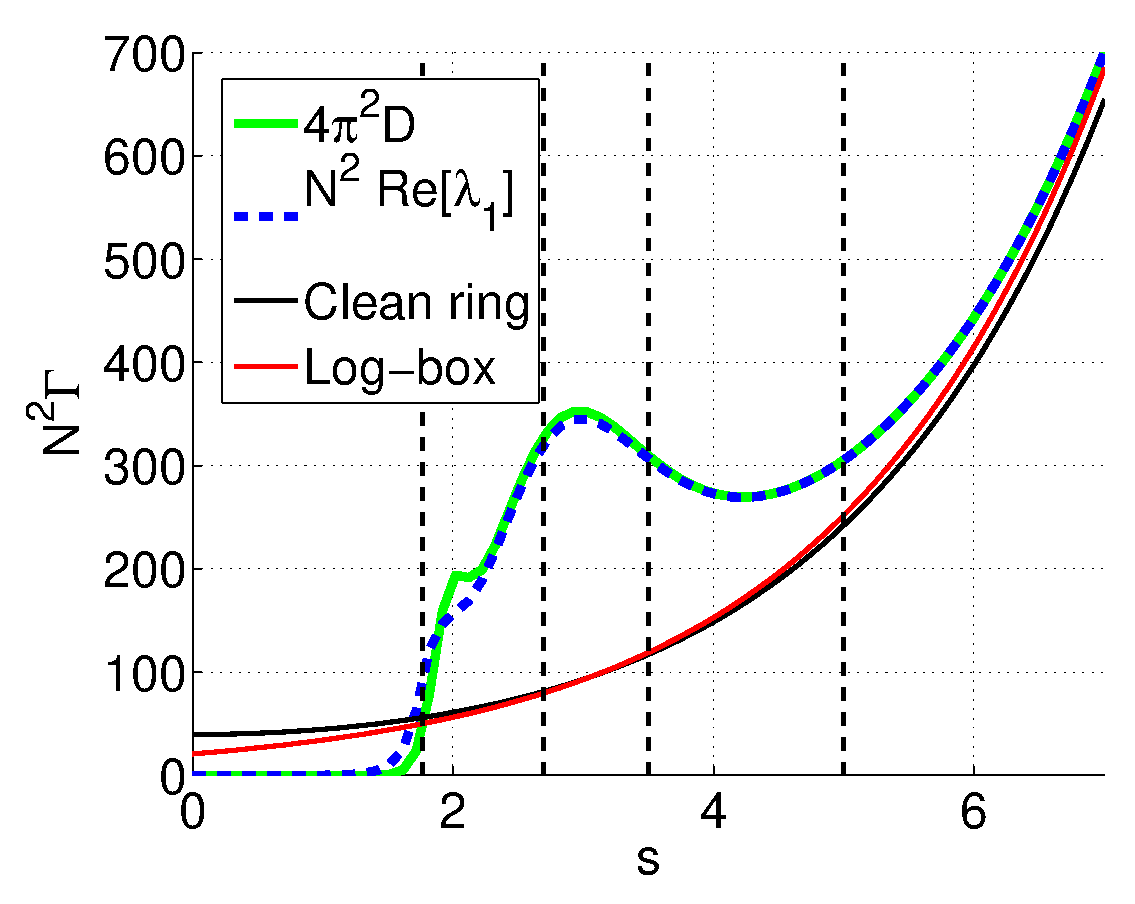
\includegraphics[height=5cm]{/Figs/gap_D_sigma5_N_1000.eps}
\caption{The real part of the gap of the complex spectrum $\Gamma = \text{Re}[\lambda_1]$ vs. $s$ for $N=1000$ sites and log-box field disorder with $\sigma=5$.
The non monotonic dashed blue line was obtained by numerically diagonalization, 
whereasthe solid green was obtained by calculating the diffusion coefficient as in \cite{nes}.
The monotonic lines correspond to the limits if a clean ring \Eq{e13} (black) and $s>s_{\infty}$, \Eq{e52} (red).
The vertical dashed lines from left to right are $s_{1/2},\  s_{1},\ s_{2}$ and $s_{\infty}$.    }
\label{f1}
\end{figure}
%%%%%%%%%%%%%%%%%%%%%%%%%%%%%%%%%%%%%%%%%%%%%%%%%%%%%%%%%%%%%%%%%%%%%%%%%%%%%%%%%%%%%%%%%%%%%%%%%%%%%%%%%%%%%%%%%%%%
\section{The secular equation}

By similarity transformation of~ $\bm{W}$ one obtains
%
\be{16}
\tilde{\bm{W}} \ \ = \ \ \text{diagonal}\{-\gamma_{n}\} \ + \ \text{offdiagonal}\{w_{n}\eexp{\pm s/2}  \}
\eeq
%
where the "$\pm$" are for the "forward" and "backward" transitions respectively.
Note that the statistics of the $\mathcal{E}_n$ is still hiding in the diagonal elements.
The associated symmetric matrix $\bm{H}$ is defined by setting ${s=0}$.
Then one can define a spectral determinant $S(z)$ and associated spectrum as follows:
%
\beq
S(z) \ \ = \ \ \det(z-H) \ \ = \ \ \prod_k (z+\epsilon_k)
\eeq
%
If the system is an  ${N}$-periodic infinite lattice, 
then ${\bm{W}}$ is similar to ${\bm{H}}$ by "gauge" transformation, 
hence one can regard the ${\{-\epsilon_k\}}$ as the spectrum of  an open chain.
But if the system is an ${N}$-periodic ring (periodic boundary conditions) 
then $s$ cannot be "gauged" away. 
Still there is a simple relation \cite{det1} that relates 
the spectral determinant of~$\bm{W}$ to that of~$\bm{H}$. Namely, 
%
\beq
\det(z-W) = S(z)-S_0 \ \ \equiv \ \ \prod_k (z+\lambda_k) 
\eeq
%
where
%
\beq
S_0 \ \ = \ \ 2\left[\cosh\left(\frac{Ns}{2}\right)-1\right]  \prod_n w_n
\eeq
%
The roots ${z=-\lambda_k}$ have real negative part, but may be complex in general.
The lowest eigenvalue ${\lambda_0=0}$ corresponds to the non-decaying 
non-equilibrium steady state (NESS). It is implied that 
%
\beq
S(0)=S_0 \ \ \ \ \ \ \ \text{implication of conservativity}
\eeq
%
We emphasize that the latter property is not true for a general 
non-Hermitian matrix, neither is the "positivity" of the ${\lambda_k}$.  
This has far reaching implications: in particular it should be 
clear that the NESS is an extended state, hence it follows that 
the localization length has to diverge in the limit ${\lambda\rightarrow0}$.
This is in essence the difference between the 
conventional Anderson model (Lifshitz tails at the band floor) 
and the Debye model (phonons at the band floor).     

From the above it follows that the secular equation for the $\lambda$ 
spectrum can be written as  
%
\be{20}
\prod_k \left(\frac{z+\epsilon_k(s)}{\overline{w}}\right) \ \ = \ \ 2\left[\cosh\left(\frac{Ns}{2}\right)-1\right]
\eeq
%
where ${\overline{w}}$ is the geometric average of all the rates.
The affinity~$s$ affects both the $\epsilon_k$ and the right hand side.

%%%%%%%%%%%%%%%%%%%%%%%%%%%%%%%%%%%%%%%%%%%%%%%%%%%%%%%%%%%%%%%%%%%%%%%%%%%%%%%%%%%%%%%%%%%%%%%%%%%%%%%%%%%%%%%%%%%%
\section{The real spectrum}

The main observation regarding the real spectrum $\epsilon_k$ of the associated symmetric matrix $\bm{H}$ 
is that for $s<s_{\infty}$ it is gapless and for $s>s_{\infty}$ it is gapped.
This can be seen both in the spetcral density and in the electrostatic potential along the real axis. Recall that  $\rho(\epsilon)\sim \epsilon^{\mu-1}$.
Consider first the case $\alpha \gg 1$, the percolation aspect is absent and $\mu=\mu_s$.
The simplest case is for $s>s_{\infty}$, where a gap opens up at $\epsilon_0 = e^{(s-\sigma)/2}$ and the spectral density is distributed log-box,
$\rho(\epsilon) = {N}/{\sigma \epsilon} $.
This holds as long as   $\alpha\gg 1$. The interesting case 
is when  $\alpha \lesssim 1$ and $s<s_{\infty}$, 
now there is a crossover in the spectrum between two anomalous behaviours. 
The bottom of the band is detemined by~${\mu_s}$ 
and the top of the band  by  ${\mu_{\alpha}}$, as show in  \Fig{fig2}.
As $\alpha$ decreases, the $\mu_s$  determined region becomes smaller.
%
This crossover is analogous to regular diffusion, where there  is a crossover from short time, diffusion limited spreading to long time drift limited spreading. 
In our case the crossover is from low energy (long time) sliding ($\mu_s$) to high energy (short time) percolation limited diffusion $\mu_{\alpha}$.

\begin{figure}
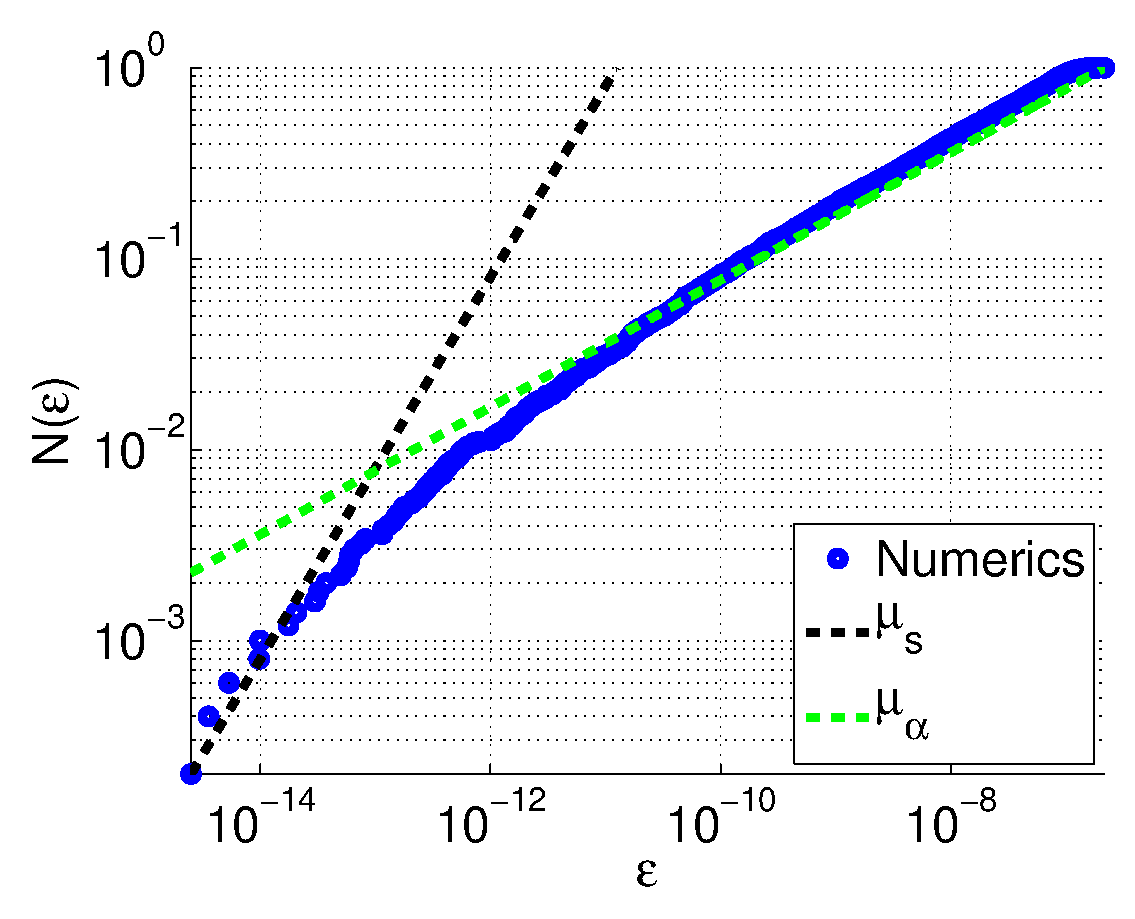
\includegraphics[height=5cm]{/Figs/N_E_0}
\caption{
A represantitive case for anomalous diffusion. 
The integrated density of states is shown for $\mu_{\alpha}=1/3$ and $\mu_s = 1$, $\sigma=2$ and  $N=5000$ sites.
The blue points are are results of numerical diagonalization. 
There is a crossover in the spectrum from sliding (dashed black line corresponds to $\mu_s$ ) to percolation  (dashed green line corresponding to  $\mu_{\alpha}$).
}
\label{fig2}
\end{figure}
%%%%%%%%%%%%%%%%%%%%%%%%%%%%%%%%%%%%%%%%%%%%%%%%%%%%%%%
%%%%%%%%%%%%%%%%%%%%%%%%%%%%%%%%%%%%%%%%%%%%%%%%%%%%%%%%%%%%%
\section{Electrostatics}

In order to get an insight into the secular equation we 
define an "electrostatic" potential as follows:
%
\be{22}
\Psi(z) \ \ = \ \ \sum_k \ln\left(\frac{z-\epsilon_k}{\overline{w}}\right) \ \ \equiv \ \ V(x,y)+iA(x,y)
\eeq
%
where ${z=x+iy}$.
 Note that compared with \Eq{e16} 
we have flipped the sign convention (${z\mapsto -z}$).
The potential for a given charge distribution $\rho(x)$ is 
${V(x,y)=\frac{1}{2} \int \ln \left[(x-x')^2 + y^2\right] \rho(x')dx'} $
and along the real axis 
%
\be{23}
V(\epsilon) =  \int \ln \left(\epsilon-x \right) \rho(x)dx 
\eeq
%
The constant ${V(x,y)}$ curves correspond to potential contours,
along which $|S(z)|$ is constant, and the constant ${A(x,y)}$ curves corresponds 
to stream lines, along which the phase of $S(z)$ is constant. 
The derivative $\Psi'(z)$ corresponds to the field, which can be regarded as 
either electric or magnetic field up to a 90deg rotation.       
Using this language the secular equation takes the form
%
\beq
V(x,y)=V(0); \ \ \ \ A(x,y)=2\pi*\text{integer} 
\eeq
%
Namely the roots are the intersection of the field lines with the 
potential contour that goes through the origin. From the preceding section
we know that the potential at the origin is 
%
\beq
V(0) \ \ = \ \ \ln\left[2\cosh\left(\frac{Ns}{2}\right)-2\right]
\eeq
%
From a straightforward electrostatic calculation we find 
that for a charge density that is given by \Eq{e3} with some cutoff $\epsilon_c$,
the derivative of the electrostatic potential at the origin is 
given by (see supplementary material for derivation)
%
\be{19}
V'(0) =\lim_{\epsilon\to 0^+}\mu \left(\frac{ \epsilon}{\epsilon_c}\right)^{\mu} \pi \cot(\pi \mu)
\eeq
%
Indicating that the sign changes from positive to negative at $\mu=1/2$.

Let us make a few observations regarding the potential $V(\epsilon)$ along the real axis.
For an illustration see \Fig{f}. Clearly if the envelope of $V(\epsilon)$ is above 
the $V=V(0)$ line, then the spectrum is real, and the $\lambda_k$ are roughly 
the same as the $\epsilon_k$, shifted a bit to the left. 
The second observation is that the envelope of $V(\epsilon)$ is positive 
in segments where the $\epsilon_k$ forms a quasi-continuum. 
This follows from the observation that $(1/N)V(\epsilon)$ equals 
the inverse localization length \cite{Shnerb1}.
% 
In the case under study the quasi-continuum starts at ${\epsilon_s=0}$ 
for ${s<s_{\infty}}$ (\Fig{f}), and at finite ${\epsilon_s}$ for ${s>s_{\infty}}$ (\Fig{figWeak}).
If follows that the threshold $s_c$ for getting a complex quasi-continuum 
is either ${V'(0)<0}$ or ${V(\epsilon_s)<V(0)}$ respectively. 
In the former case it follows from \Eq{e19} that ${s_c=s_{1/2}}$.

\begin{figure}
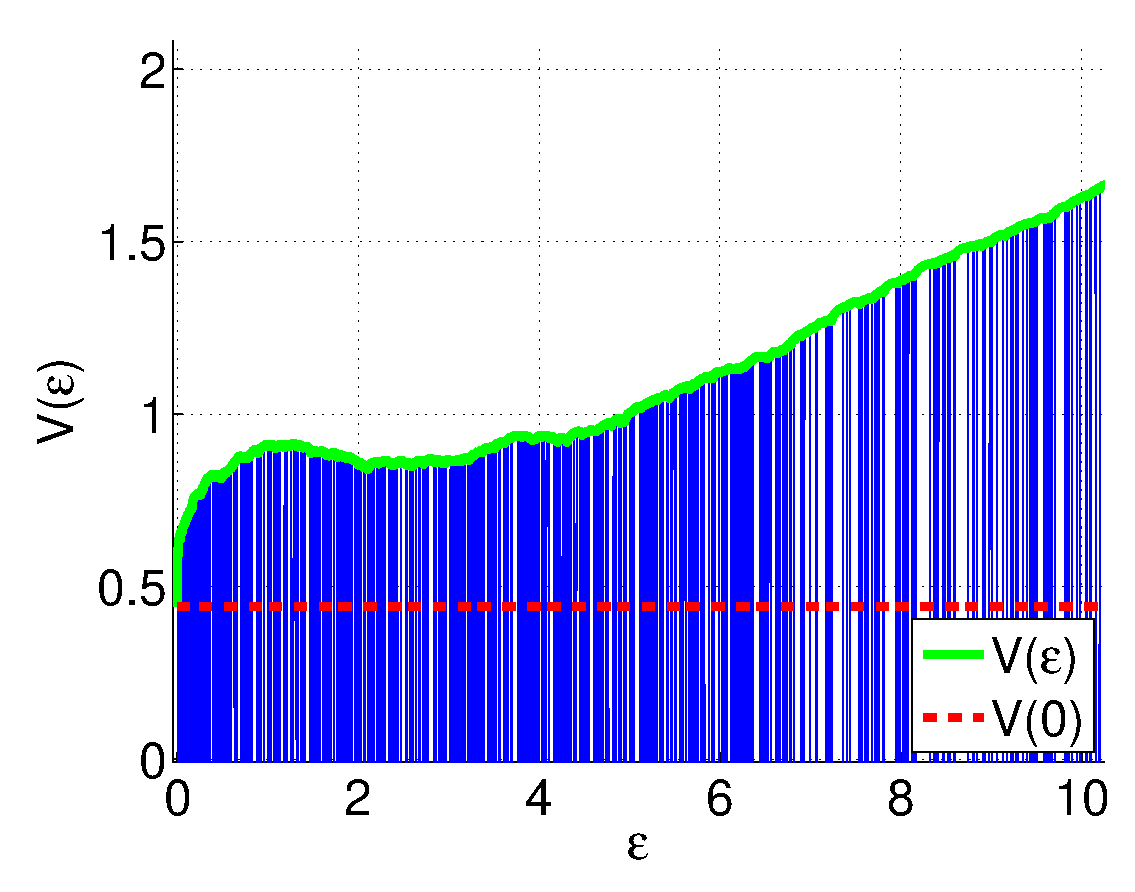
\includegraphics[height=5cm]{/Figs/V_E_localized.eps}
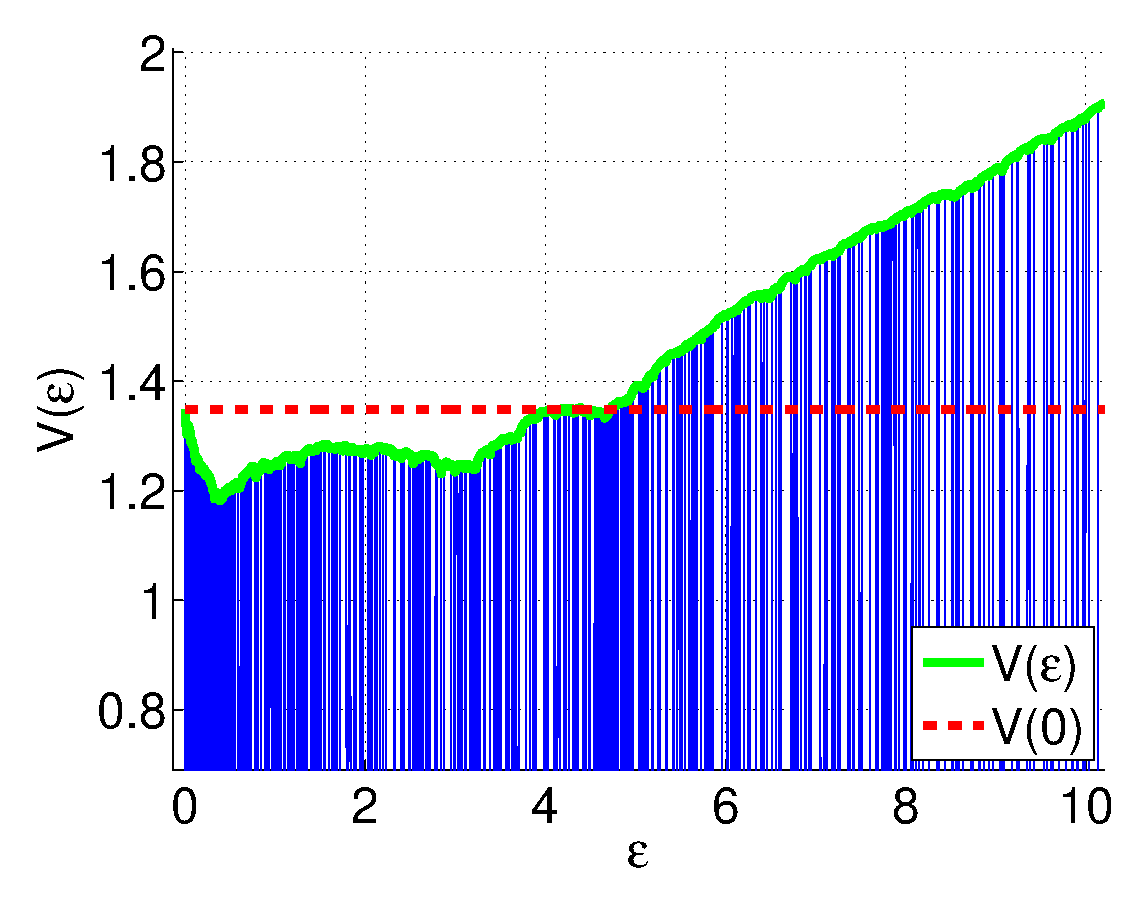
\includegraphics[height=5cm]{/Figs/V_E_delocalized.eps}
\caption{
The electrostatic potential along the real axis. Top panel: $s<s_{1/2}$, the spectrum is real and localized.
Bottom panel: $s>s_{1/2}$, the bottom of the band is delocalised and complex. 
Here $N=1000$, $\sigma = 5$ for the top panel we used $s=s_{1/2}/2$, for the bottom panel, $s=s_1$.}
\label{f}
\end{figure}

%%%%%%%%%%%%%%%%%%%%%%%%%%%%%%%%%%%%%%%%%%%%%%%%%%%%%%%%%%%%%%%%%
\section{Determination of $s_c$ - white vs sparse disorder }

The simplest case to exhibit a crossover to a complex spectrum is that of a single defect. 
There are two types of defects, either in the couplings $w_n$ or in the fields $\mathcal{E}_n$. 
The details are slightly different, but the analysis is essentially the same. 
Consider first a single defect in the couplings, such that  $w_1 = g, \ w_{n\neq1}=1$ where $g\ll1$. 
The spectrum of the associated Hermitian matrix $\bm{H}$ 
is composed of a single state $\epsilon_1$ and a quasi-continuum which begins at $\epsilon_s > \epsilon_1$.
The single state is pushed down from the quasi-continuum such that \rmrk{(From numerical experiments, I still don't have the exact physical argument)}
$\epsilon_s = \epsilon_1/g = s^2/4g$.
% $\epsilon_s = v^2/4D + D\pi^2/N^2 $ and a single
%state $\epsilon_1 \approx s^2/4g$ that is pushed down from the continuum (but not zero). 
%To obtain $\epsilon_1$ we use the same argument as in the continuum derivation. This ground state should be $v^2/4D$,  we assume that the local diffusion coefficient is $gD$ but that the drift velocity is not affected.
%
The potential at $\epsilon_s$ due to the continuum is zero and the potential there, 
generated by $\epsilon_1$ is  (Assuming $s\ll1, \ N\gg 1$)
%
\beq
V(\epsilon_s) = \ln \left|\frac{\epsilon_s-\epsilon_1}{g}\right| \approx  \ln \left(\frac{s^2}{4g^2}\right) 
\eeq
%
Complex eigenvalues appear when $V(\epsilon_s) < V(0)$, leading to the equation for $s_c$
%
\beq
1+\frac{1}{2}\left(\frac{s}{2g}\right)^2 =\cosh\left(\frac{Ns}{2}\right)
\eeq
%
The exact equation, derived from the continuum limit (see supplementary material) is 
%
\beq
\sqrt{1+ \left(\frac{s}{2g}\right)^2}  \ = \  \cosh\left(\frac{Ns}{2}\right)
\eeq
%
If there are $M$ defects ("sparse" disorder) then there are $M$ states that are separated from the continuum
and they are equal in the vicinity of $s_c$ (numerically verified), so
${V(\epsilon_s) \approx M \ln(s^2/4g^2)}$ and the equation for $s_c$ is 
%
\beq
\sqrt{1+ \left(\frac{s}{2g}\right)^{2M}}  \ = \  \cosh\left(\frac{Ns}{2}\right)
\eeq
%

For a defect in the stochastic field, all of the transition rates are $e^{\pm s/2}$ except for a single bond where the rates are $e^{\pm(s-\sigma)/2}$. As a result there are 4 different decay rates 
%
\beq
\gamma_0 &=& 2e^{-\sigma/2} \cosh(s/2),\\
\gamma_1 &=& 2\cosh(s/2)\\
\gamma_2 &=&e^{s/2}+e^{-(s-\sigma)/2}\\
\gamma_3 &=&e^{(s+\sigma)/2}+e^{-s/2} 
\eeq
%
The spectrum $\epsilon_k$ of the symmetric matrix $\bm{H$} is 
composed of a continuum in the range $2\cosh(s/2)\pm 2$ 
with three additional states: $\gamma_0$ is beneath the continuum while $\gamma_2, \gamma_3$ are above the continuum by a factor of $\exp(\sigma/2)$.
%
As in the previous model, the continuum contributes zero to the potential at $\epsilon_s$.
The charges above the continuum contribute ${V(\epsilon_s) = \ln\gamma_2 + \ln \gamma_3 \approx \sigma}$. From  the requirement ${V(\epsilon_s)<V(0)}$, one gets 
%
\beq
s_c = \frac{2\sigma}{N} 
\eeq
%

%%%%%%%%%%%%%%%%%%%%%%%%%%%%%%%%%%%%%%%%%%%%%%%%%%%%%%%%%%%%%%%%%
\section{Complexity diminishes the real gap for $s >  s_{\infty}$ }
%
As we discussed, the spectrum of $\bm{H}$ is gapped for $s>s_{\infty}$, with a quasi continuum beginning at 
${\epsilon_0 \propto \exp[(s-\sigma)/2]}$.
However, the gap of the complex spectrum is diminished and is given by the expression
%
\be{52}
\text{Re}[ \lambda_1 ]   \ \approx \ \frac{ 2\pi^2 }{N^2} e^{s/2-s_{1/2}}\cosh\left(\frac{\sigma}{2}\right)
\eeq
%
The gap grows with $s$ as expected, but diminishes as $1/N^2$.
To obtain this expression we use the 2D electrostatics picture previously described.
The density of states is $\rho(\epsilon) = N/\sigma\epsilon$, where $\epsilon \in [a,b]$ and 
${a=\exp[(s-\sigma)/2],  \ b =  \exp[(s+\sigma)/2]}$. The equipotential contour, $V(x,y) =V(0)$ is approximately a parabola near the origin (see \Fig{figWeak} for an illustration), so $x=Cy^2$ should solve the equation. On the other hand, $V(x,y)$ can be expanded near the origin
%
\beq
V(x,y) \ \ &=& \ \ \frac{1}{2}\int_a^b \ln \left((x-X)^2 + y^2\right) \rho(X) dX \\
%&\approx & \int_a^b \left(\ln(X) -\frac{x}{X} + \frac{1}{2} \frac{y^2}{X^2} \right)\rho(X) dX = \\
\ &\approx & \ C_0 - C_1 x +\frac{1}{2}C_2y^2 
\eeq
%
where the coefficients $C_n$ are defined 
%
\beq
C_n = \int_a^b \frac{1}{x^n}\rho(x)dx
\eeq
%
Notice that $C_0 = V(0), \ \ C_1 = E_x(x,0)$.
Since we are interested in the contour $V(x,y) = V(0,0)$, we obtain
%
\be{48}
x = \frac{1}{2}\frac{C_2}{C_1} y^2 
\eeq
%
For the given density of states we obtain 
%
\beq
C =  \frac{1}{2}\frac{C_2}{C_1} = \frac{1}{2} e^{-s/2}\cosh\left(\frac{\sigma}{2}\right) 
\eeq
%
The gap is determined by integrating the electric field, $\vec{E}(x,y) = - \vec{\nabla } V$, along the parabola of \Eq{e48}
%
\beq
\int_{0}^{\sqrt{Re[\lambda_1]/C}} \left|\vec{E}(x,y)\right| dy \ = \ 2\pi
\eeq
%
This is equivalent, through Cauchy Riemann, to the requirement $A(Re[\lambda_1],0)=2\pi$.
%
The integrand is approximated by $|\vec{E}(x,y)| \approx |\vec{E}(0,0)|$ by which we obtain
an estimate for the gap
%
\beq
\text{Re}[ \lambda_1 ] \approx \frac{4\pi^2 C}{ \left|\vec{E}(0,0) \right|^2} \ = \ \frac{ 2\pi^2 }{N^2} e^{s/2-s_{1/2}}\cosh\left(\frac{\sigma}{2}\right)
\eeq
%

The same derivation can be repeated for density of states characterized by the exponent $\mu$ to obtain (see supplementary)
%
\beq
\text{Re}[\lambda_1] \sim \frac{1}{N^2}\frac{(\mu-1)^3}{\mu^2(\mu-2)}
\frac{1- \left(\frac{a}{b}\right)^{\mu-2}}{\left(1- \left(\frac{a}{b}\right)^{\mu-1}\right)^3}b^{1-2\mu}
\eeq
%


The potential along the real axis for the log-box case can be computed analytically
%
\be{43}
 V(\epsilon) \  &=& \ 
 \ln(| \epsilon - b|) \ln\left(\frac{b}{\epsilon}\right) + \ln(|\epsilon-a|) \ln \left(\frac{\epsilon}{a}\right) +\\
 &+&
   \text{Li}_2\left( 1 -\frac{b}{\epsilon}\right) + \text{Li}_2\left( 1-\frac{a}{\epsilon}\right) 
\eeq
%
\begin{figure}[h!]
 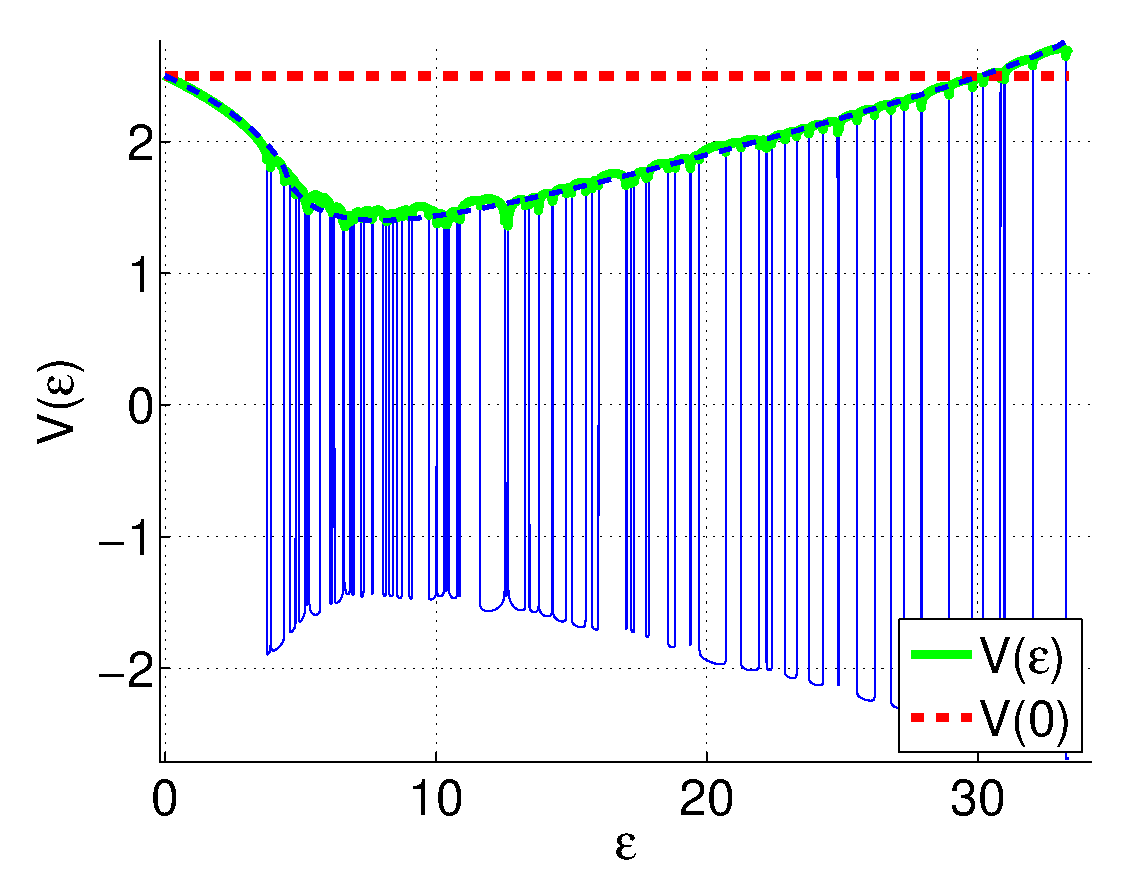
\includegraphics[width=7cm]{/Figs/V_E_s_inf}
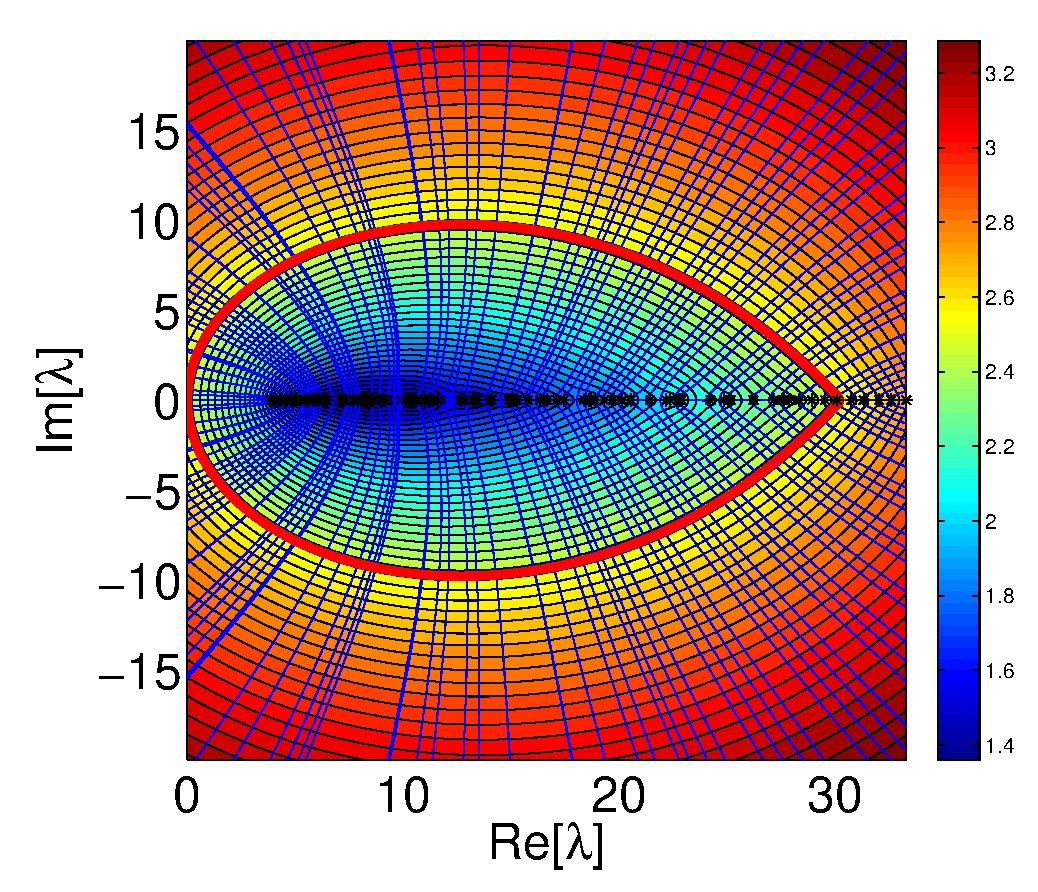
\includegraphics[width=8.5cm]{/Figs/electrostatics_large_S}
 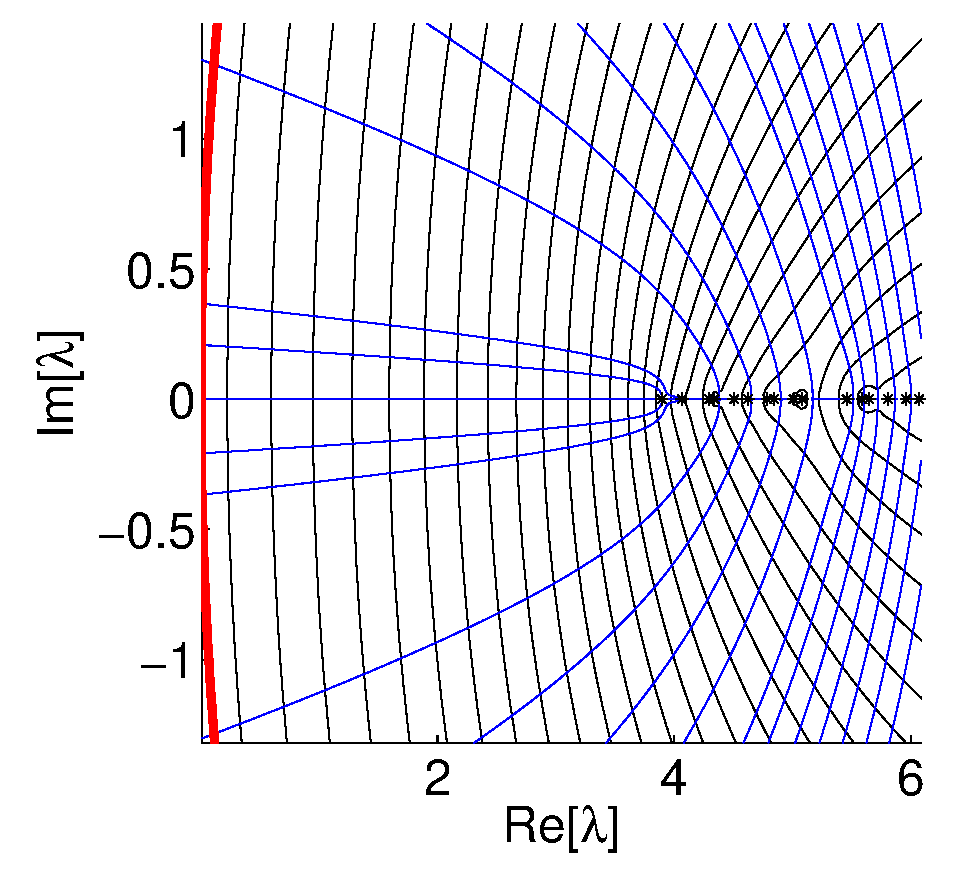
\includegraphics[width=7cm]{/Figs/electrostatics_large_S_zoom}

\caption{ Top: The electrostatic potential along the real axis, $V(\epsilon)$. The green points are the result of numerical diagonalization, the dashed blue line is the analytical result assuming $\rho=N(\sigma x)^{-1}$, \Eq{e43}. 
The stars 
indicate the position of the "charges", which are the eigenvalues of the associated Hermitian matrix, $\varepsilon_j$.
Middle: Field lines and potential of the corresponding electrostatic problem in the entire complex plane. 
The points of intersection of the field lines (thin blue lines) with the contour $V(\lambda) = V(0)$ (thick red contour) are the solutions to the secular equation. 
Bottom: Zoom in on the origin. 
The red line is the equipotential line $V(\lambda) = V(0)$.
The gap in the spectrum of $\bm{H}$  (black stars) is large, 
but the real gap in the complex spectrum, (intersection
of the contour $V=V(0)$and the first field line) diminishes as $1/N^2$.
Here $N=100$ sites, $\sigma=2$ and $s=5$.
}
\label{figWeak}
\end{figure}

%%%%%%%%%%%%%%%%%%%%%%%%%%%%%%%%%%%%%%%%%%%%%%%%%%%%%%%%%%%%%%%%%
\section{Complexity saturation for $s \gg s_{\infty}$ }


The secular equation for the eigenvalues is given by \Eq{e20}.
%
In the nonconservative case, the eigenvalues of $\bm{H}$ do not depend on $s$,
 thus raising $s$ will eventually make the entire spectrum complex. 
For a conservative matrix, however, $V(\epsilon)$ is also a function of $s$, so increasing $s$ raises $V(\epsilon)$  at the same rate.
%
Due to the conservative property, the eigenvalues of the associated hermitian martix, $\epsilon_j$ 
grow proportionaly to $e^s$. 
Increasing $s \to s+\Delta s$, we have
%
\beq
\sum_k \ln\left(\frac{z-\epsilon_k e^{\Delta s}}{\overline{w}}\right)
&=&
 \ln \left[2\cosh\left(\frac{(s+\Delta s)N}{2}\right) -2\right] \\
\sum_k \ln\left( \frac{z e^{-\Delta s} - \epsilon_k}{\overline{w}}
 \right) 
 + N\Delta s &=&
 \ln \left[2\cosh\left(\frac{sN}{2}\right) -2\right] +N\Delta s \ \ \ \ \ \ \ \ \
\eeq
%
but $z$ is just a dummy variable, so we can redefine $z := z e^{-\Delta s}$ and the equation is unchanged. Thus increasing $s$ does not change the number of complex solutions, as shown in \Fig{figCplxSat}.


%%%%%%%%%%%%%%%%%%%%%%%%%%%%%%%%%%%%%%%%%%%%%%%%%%%
To estimate the the saturation value of the fraction of complex eigenvalues, we assume $s \gg s_{\infty}$.
The eigenvalues have a log-box distribution so the potential along the real axis is 
%
\beq
V(\epsilon) \ \ &=& \ \  \int_a^b \ln|\epsilon - \epsilon'| \rho(\epsilon')d\epsilon'  =  \\
\ \ &=& \ \ \int_{-\sigma}^{\sigma} \ln \left| e^{(s+\mathcal{E})/2} - e^{(s+\mathcal{E}_c)/2}\right| \rho(\mathcal{E})d\mathcal{E} = \\
\ \ &=& \ \ \frac{N}{2\sigma}\int_{-\sigma}^{\sigma} \ln \left| e^{(s+\mathcal{E}_c)/2} - e^{(s+\mathcal{E})/2}\right| d\mathcal{E}
\eeq
%
Define $\mathcal{E}_c$ such that the eigenvalues with $\mathcal{E}$ 
in the range ${-\sigma < \mathcal{E} < \mathcal{E}_c}$ are complex, $\mathcal{E}_c$ is determined by the equation ${V(\epsilon=e^{(s+\mathcal{E}_c)/2}) =  V(0) = sN/2}$, leading to 
%
\beq
\int_{-\sigma}^{\sigma} \ln \left| e^{(s+\mathcal{E})/2} - e^{(s+\mathcal{E}_c)/2}\right| d\mathcal{E}  \ \ = \ \ 0 
\eeq
%
Clearly, $\mathcal{E}_c$ depends only on $\sigma$ (\Fig{figCplxSat}).
The fraction of complex eigenvalues  is just 
%
\be{101}
n =\frac{ \int_a^{\epsilon_c}  \frac{1}{ \epsilon} d\epsilon}{ \int_a^{b}  \frac{1}{ \epsilon} d\epsilon} = 
\frac{1}{\sigma}\ln\left( \frac{\epsilon_c}{a} \right) = 
\frac{\mathcal{E}_c + \sigma}{2\sigma}
\eeq
%
If instead of a lattice we had a continuous problem and the field disorder was "white noise", 
the electrostatic potential would be different, as in \cite{odh3}. 
It has a peculiar trait that  $V(\epsilon \to \infty) = \text{const}$. the potential reaches a constant value,
implying that the entire spectrum becomes complex at once (\Fig{figCplxSat}).


%%%%%%%%%%%%%%%%%%%%%%%%%
\begin{figure}[h]
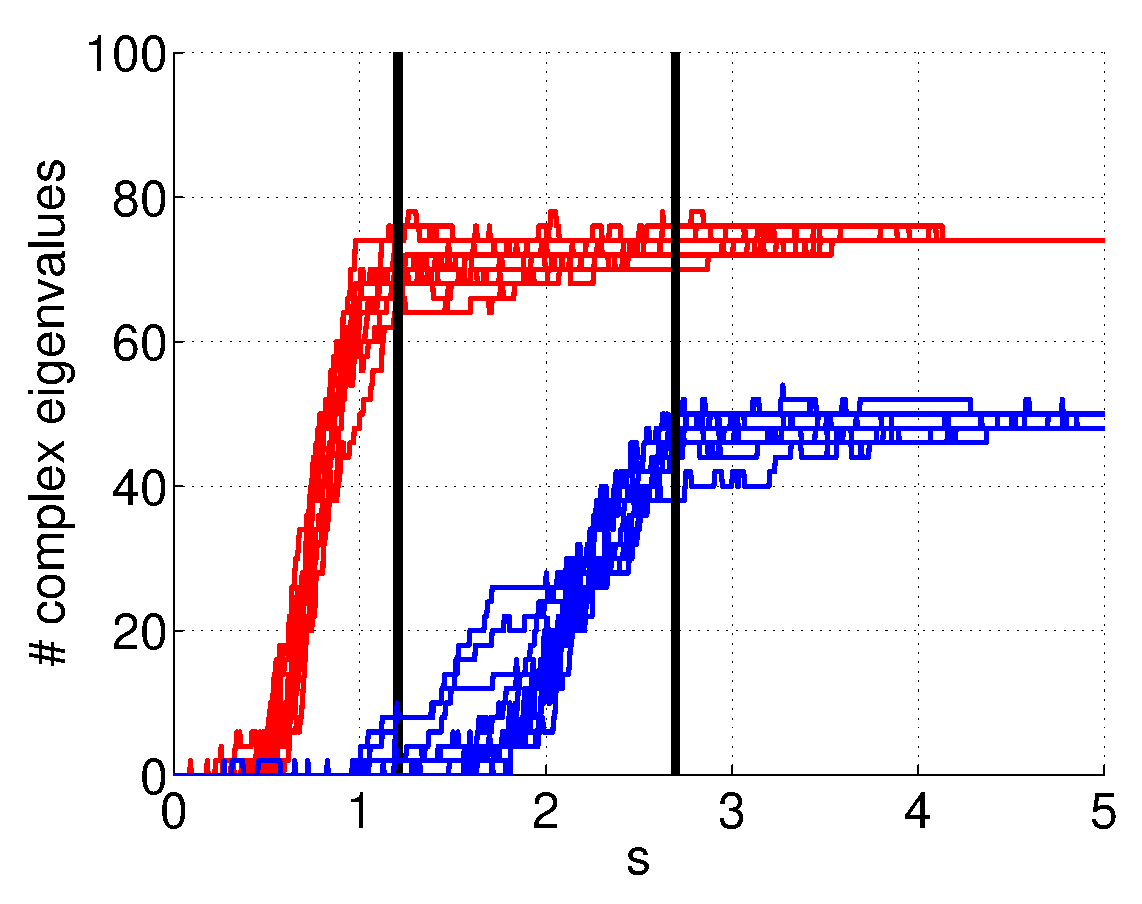
\includegraphics[height=5cm]{/Figs/num_cplx.eps}
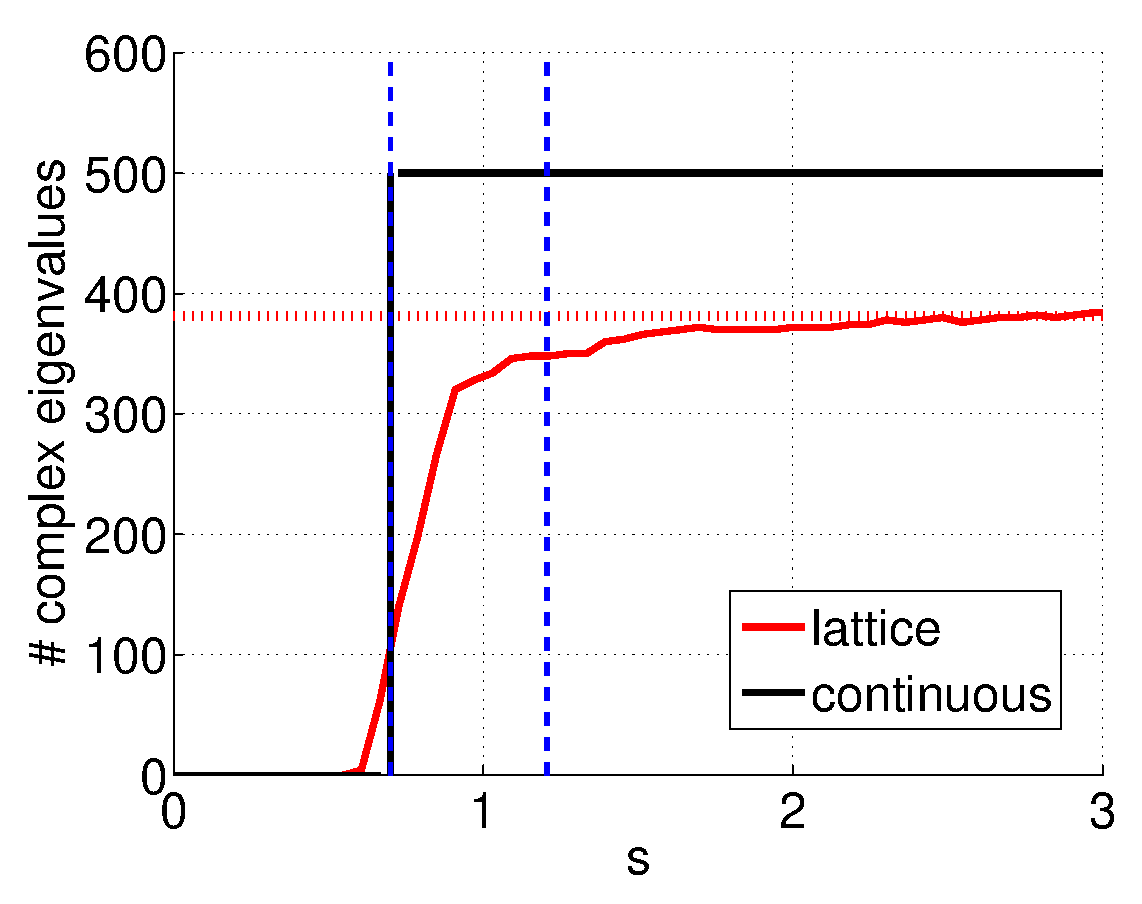
\includegraphics[height=5cm]{/Figs/numComplex_500}
\caption{Top: Number of complex eigenvalues vs. $s$ for $N=100$ sites. 
Each red line corresponds to a different 
realisation of field disorder with $\sigma=3$ (red) and $\sigma=5$ (blue), and $\alpha=\infty$. The black vertical lines are at values of $s_1(\sigma)$ at which the sliding transition occurs.
Bottom: Number of complex eigenvalues vs. $s$ for $N=500$ sites and $\sigma=5$ (red)
vs. the result of the continuous, white noise, problem (black step function). 
The vertical dashed lines are $s_{1/2}$ and $s_1$. The dotted horizontal red line is the estimated saturation value, \Eq{e101}. }
\label{figCplxSat}
\end{figure}


\clearpage

%%%%%%%%%%%%%%%%%%%%%%%%%%%%%%%%%%%%%%%%%%%%%%%%%%%%%%%%%%%%%%%%%
\hide
{\section{Garbage}

\[ V(R) = \int_{0}^{x_c} \rho(x) \ln|x-R| dx \]

\[ V(R) = -\int_{0}^{x_c} \frac{(x/x_c)^{\mu}}{x-R} dx \]

More convenient to consider

\[ -\frac{1}{2} \int_{-u_c}^{u_c} \frac{ u^{2\mu+1} }{u^2-R} dx \]

For ${\mu=0}$ we recover the log potential of a point charge.
For ${\mu>0}$ the singularity is smeared and  ${V(0)}$ becomes finite.

\[ V(0) = - \frac{1}{\mu}  \]

In general ${x_c}$ is the border between the ${x^{\mu}}$ region 
and the "clean ring" region that extends up to the upper band edge.  
Accordingly ${V(0)}$ is shifted upwards.   

For ${\mu=1/2}$ we get  

\[V(R) = \{ (R/x_c)^{1/2}-1; \ \ \ \ -1(R>0) \} \] 

For general ${\mu}$ we need the derivative. 
For ${R<0}$ the calculation is straightforward

\[ V'(R<0) = -\int_{-u_c}^{u_c} \frac{ u^{2\mu+1} }{(u^2-R)^2} dx \]
 
leading to infinite slope at ${R=-0}$ for ${\mu<1}$.
Only for ${\mu>1}$ the left slope ${V'(-0)}$ becomes finite and continuous.

The expressions for ${V'(+0)}$ required regolarization in the regime ${R>0}$, 
leading for any ${\mu}$ to a finite-slope result

\[ V'(+0) = -\Gamma(2\mu-2) \frac{1}{x_c} \]

For Math see

Computing the Hilbert Transform of the Generalized Laguerre and Hermite Weight Functions 
http://link.springer.com/article/10.1023%2FA%3A1021915128433

The slope change sign at ${\mu=1/2}$, 
hence for ${\mu>1/2}$ the minimum of ${V(R)}$ is to the right of ${R=0}$. 
 }


%%%%%%%%%%%%%%%%%%%%%%%%%%%%%%%%%%%%%%%%%%%%%%%%%%%%%%%%%%%%%%%%%%%%%%%%%%%%%%%%%%%%
%%%%%%%%%%%%%%%%%%%%%%%%%%%%%%%%%%%%%%%%%%%%%%%%%%%%%%%%%%%%%%%%%%%%%%%%%%%%%%%%%%%%
\clearpage
\bibliography{neg_bib.bib}{}
\bibliographystyle{ieeetr}


%%%%%%%%%%%%%%%%%%%%%%%%%%%%%%%%%%%%%%%%%%%%%%%%%%%%%%%%%%%%%%%%%%%%%%%%%%
%%%%%%%%%%%%%%%%%%%%%%%%%%%%%%%%%%%%%%%%%%%%%%%%%%%%%%%%%%%%%%%%%%%%%%%%%%

\section*{Acknowledgements}

This research has been supported by  by the Israel Science Foundation (grant No. 29/11).


\hidea{
\section*{Author contributions statement}

Both authors have contributed to this article. 


\section*{Additional information} 

% Reprints and permissions information is available at www.nature.com/reprints\\
The authors declare that they have no competing financial interests.
% Correspondence and requests for materials should be addressed to avardi@bgu.ac.il or dcohen@bgu.ac.il

}
%%%%%%%%%%%%%%%%%%%%%%%%%%%%%%%%%%%%%%%%%%%%%%%%%%%%%%%%%%%%%%%%%%%%%%%%%%
%%%%%%%%%%%%%%%%%%%%%%%%%%%%%%%%%%%%%%%%%%%%%%%%%%%%%%%%%%%%%%%%%%%%%%%%%%


\clearpage
\subsection{Appendix - Finding the sign of $V'(0)$}

To derive \Eq{e19} we assume an integrated density of states corresponding to \Eq{e3}, 
${\mathcal{N}(\epsilon) = (\epsilon/\epsilon_c)^{\mu}}$, where $\epsilon_c$ is some cutoff due to the discreteness of the lattice.
The electrostatic potential along the real axis is given by (integration by parts of \Eq{e23})
%
\beq
V(\epsilon) &=& -  \int_0^{\epsilon_c} \frac{\mathcal{N}(x)}{x-\epsilon}dx
\eeq
and the derivative with respect to $\epsilon$ at the origin is (after integrating by parts)
%
\beq
V'(0) \ \ &=& \ \ \lim_{\epsilon\to 0^+} \int_0^{\epsilon_c} \frac{\mathcal{\rho}(x)}{x-\epsilon}dx = \\
\ \ &=& \ \ \lim_{\epsilon\to 0^+}  \frac{\mu}{\epsilon_c^{\mu}}\int_0^{\epsilon_c} \frac{x^{\mu-1}}{x-\epsilon}dx \ = \ \frac{C}{\epsilon_c}
\eeq
%
The integral converges for $\mu<1$. To cacluate $C$ we first substitute $z=x/\epsilon$, such that
%
\beq
C = \lim_{z_c\to \infty} \frac{\mu }{z_c^{\mu-1}}\int_0^{z_c}\frac{z^{\mu-1}}{z-1}dz
\eeq 
%
The integral can be written in terms of Incomplete Euler Beta functions defined as 
%
\beq
B_u(a,b) = \int_0^u x^{a-1}(1-x)^{b-1}dx
\eeq
%
However one must be careful and take only the Cauchy principal part
\beq
I  &=&  \int_0^{u}\frac{x^{\mu-1}}{x-1}dx =\\
& \ \ = \ \ & \lim_{\varepsilon \to 0} \left[ \int_0^{1-\varepsilon}x^{\mu-1}(1-x)^{-1}dx + 
\int_{1+\varepsilon}^u x^{\mu-1}(1-x)^{-1}dx \right]= \\
&=&\lim_{\varepsilon \to 0}  \left[ B_{1-\varepsilon}(\mu,0) - B_{1-\varepsilon}(1-\mu,0) \right] = \\
&=& \psi(1-\mu)-\psi(\mu) = \pi \cot(\pi \mu)
\eeq
%
where $\psi(z)$ is the digamma function and the last equality was obtained by the reflection formula. 
%
To go from the second to the third line we made the substitution $t=1/x$ and took the limit $u\to \infty$.
%
It is clear that $C$ and thus $V'(0^+)$ changes sign from positive to negative at $\mu=1/2$.\\
%
%\beq
%V'(0^+) =\lim_{R\to 0^+} \frac{ R^{\mu}}{x_c^{\mu}} \pi\mu \cot(\pi \mu)
%\eeq

%%%%%%%%%%%%%%%%%%%%%%%%%%%%%%%%%%%%%%%%%%%%%%%%%%%%%%%%
\subsection{Sliding transition - the definition of $s_{\mu}$}

\subsection{ The similarity transformation (definition of H)} 

\subsection{The formula for the spectral determinant}

\subsection {Clean ring}

\subsection{ Ring with weak link "$g$"}

\subsection{ Ring with sparse disorder}

\subsection{ Ring with white disorder (�French�) }

\subsection{ Step by step electrostatics}


\end{document}
%%%%%%%%%%%%%%%%%%%%%%%%%%%%%%%%%%%%%%%%%%%%%%%%%%%%%%%%%%%%%%%%%%%%%%%%%%
%%%%%%%%%%%%%%%%%%%%%%%%%%%%%%%%%%%%%%%%%%%%%%%%%%%%%%%%%%%%%%%%%%%%%%%%%%


